\documentclass[resume]{subfiles}


\begin{document}
\section{File system}
<<<<<<< Updated upstream
\subsection{Génération}
Squelette de rootfs dans \verb!workspace/nano/buildroot/system/skeleton!. Il est ensuite copié dans \verb!buildroot/output/target! et les fichiers nécessaires y sont ensuite ajoutés.\\
Une fois que tous les fichiers sont ajoutés, une image \verb!rootfs.xxx! est créé (xxx est ext4, squashfs, etc...)
=======

\subsection{}

\subsection{1. De connaître les différents types de systèmes de fichiers ainsi que leurs applications}

Pour les systèmes embarqués, il existe deux catégories de systèmes de fichiers :
- Volatiles en RAM
- Persitants sur des Flash (NOR et de plus en plus NAND)

Deux technologies principales sont disponible sur les Flash :  
- soit les MTD (Memory Technology Device)
- les MMC/SD-Card (Multi-Media-Card / Secure Digital Card)

\begin{figure}[H]
    \centering
    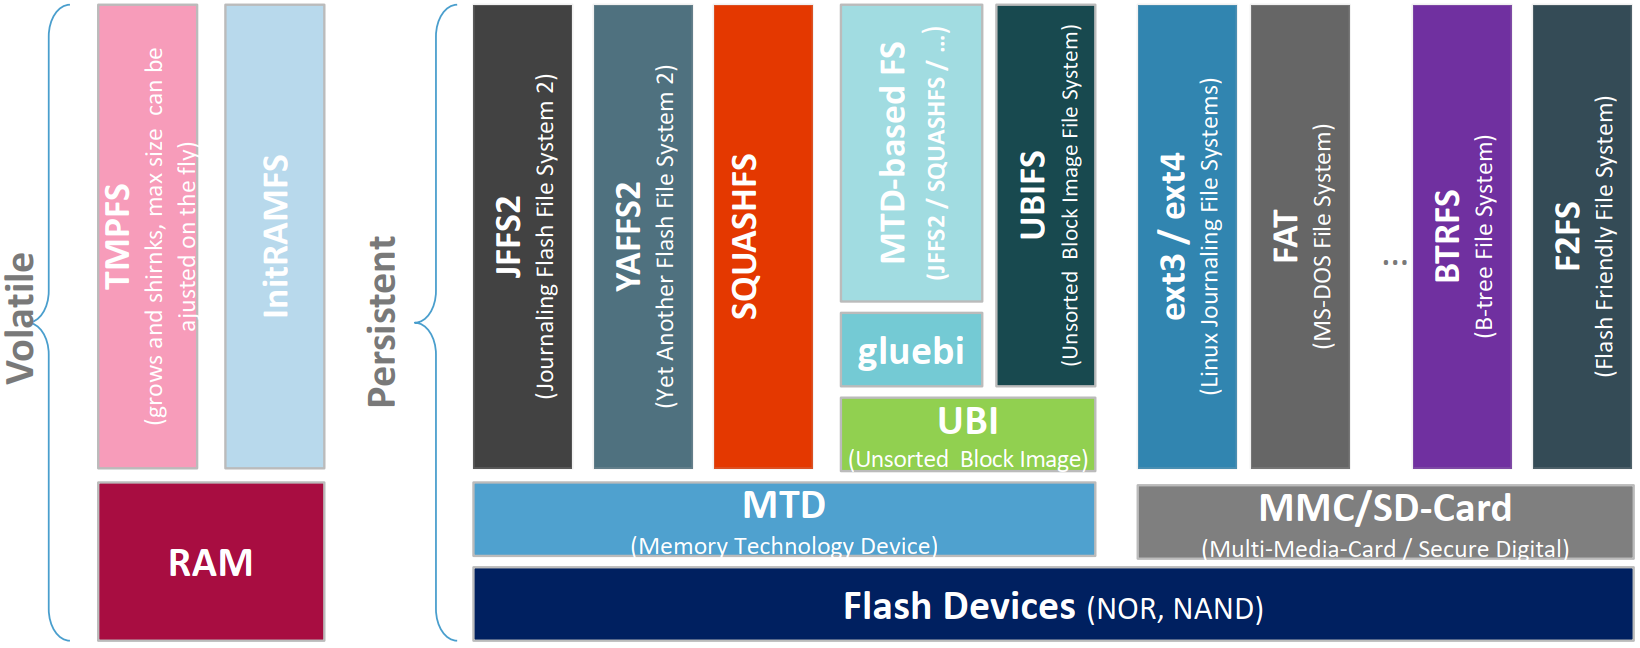
\includegraphics[width=0.7\textwidth]{Figures/fileSystem/fileSystemType.PNG}
    \caption{FS type}
    \label{fig:fileSystemType}
\end{figure}

\subsubsection{Choix d'un FS}
\begin{figure}[H]
    \centering
    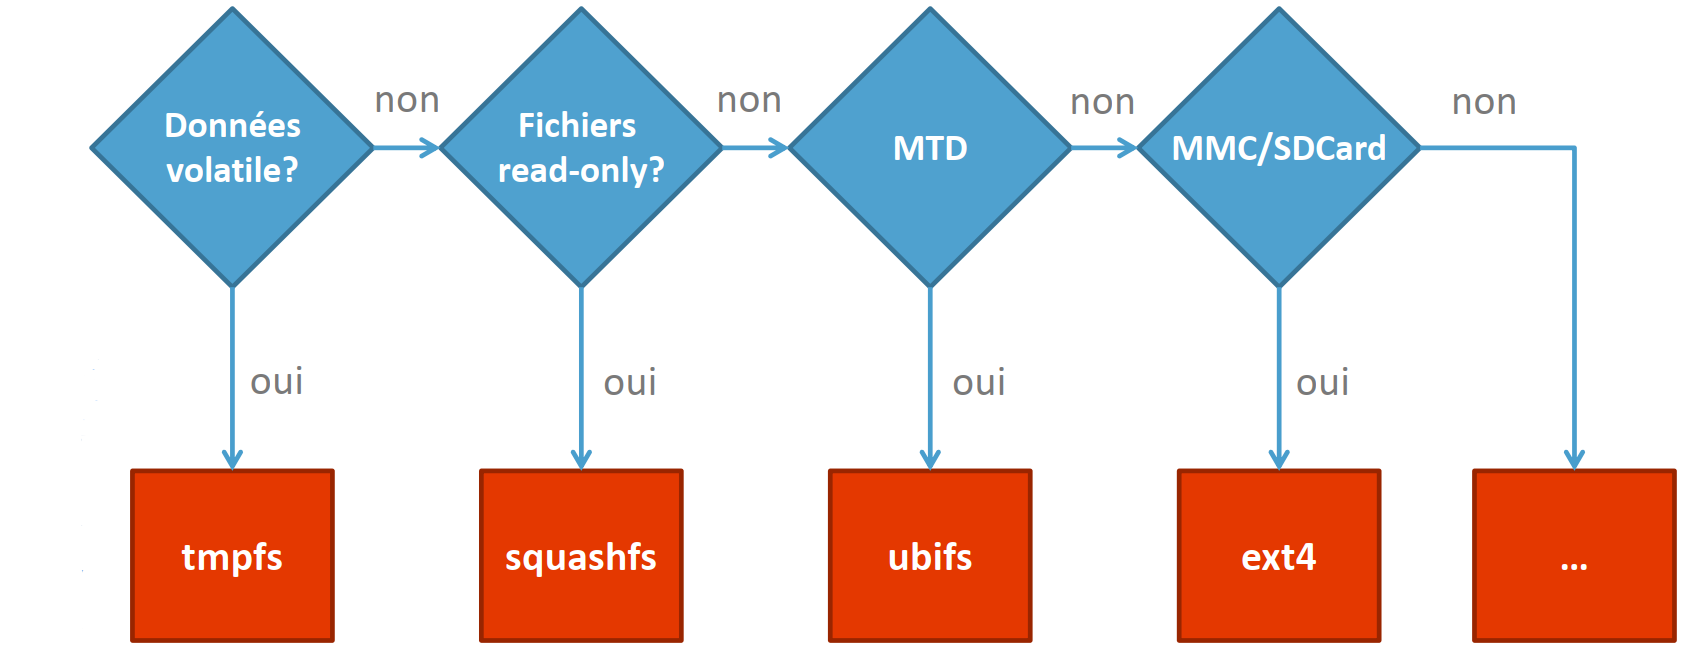
\includegraphics[width=0.7\textwidth]{Figures/fileSystem/fileSystemChoice.PNG}
    \caption{FS type}
    \label{fig:fileSystemChoice}
\end{figure}

\subsection{2. De connaître les caractéristiques des filesystems ext2-3-4, ainsi que les commandes associées}


\subsection{3. D’expliquer les différents « files systems » utilisés dans les systèmes embarqués (ext2-3-4, BTRFS, F2FS, NILFS2, XFS, ZFS, …)}


\subsection{4. Expliquer les « files system » de type Journal, B_Tree/CoW, log filesystem}


\subsection{5. De connaître les caractéristiques du filesystem Squashfs, ainsi que les commandes associées}


\subsection{6. De connaître les caractéristiques du filesystem tmpfs, ainsi que les commandes associées}


\subsection{7. De connaître les caractéristiques du filesystem LUKS, ainsi que les commandes associées}


\subsection{8. Savoir expliquer la gestion des clés de LUKS 42}


\subsection{9. De connaître les caractéristiques du filesystem InitramFS, ainsi que les commandes associées}


\subsection{10. De savoir créer un initramFS}
>>>>>>> Stashed changes


\end{document}